%\documentclass[MTRX3700report.tex]{subfiles}
\documentclass[11pt,a4paper]{article}
% Dpak
% HARDWARE DESIGN
\usepackage{color}
\usepackage{floatrow}
\usepackage{graphics}
\usepackage{graphicx}
% Table float box with bottom caption, box width adjusted to content
\newfloatcommand{capbtabbox}{table}[][\FBwidth]

\begin{document}
  \textcolor{red}
  {
  \textit{Give a detailed description of the design of hardware. The description should include mechanical drawings, location diagrams, electrical circuit schematics, circuit simulation or test results, PCB overlays, wiring diagrams, connector pinout lists, pneumatic/hydraulic circuit diagrams}
  }
  \\The project includes a wide array of hardware types, each with specific requirements to be interfaced with in software and with other the other hardware components. This section will seek to outline the requirements of the individual components used, as well as the scheme with which they were interfaced with each other.

  \subsection{Scope of the Jousting Robot's System Hardware}
    The jousting robot, being composed of 2 interacting systems, namely the Commander and Mobile Robot, has a hardware requirement that was also split into two.
    The Commander hardware and Mobile Robot hardware will be here discussed separately to highlight the differences.
  \subsection{Hardware shared between Commander and Mobile Robot}
    The Commander and Mobile robot function in a master/slave relatoionship and so required a common denominator of components for communication between them. These common components included the PIC18f4520 MNML microprocessor, and the Xbee communication hardware.
    \subsubsection{PIC18f4520 Microcontroller}
    The PIC18f4520 is a RISC microcontroller with harvard architecture and is well suited to embedded projects. The MNML board used provides access to the MPLABx development environment through the RJ45 connector via the ICD (in circuit debugger).

    \begin{figure}[h]
        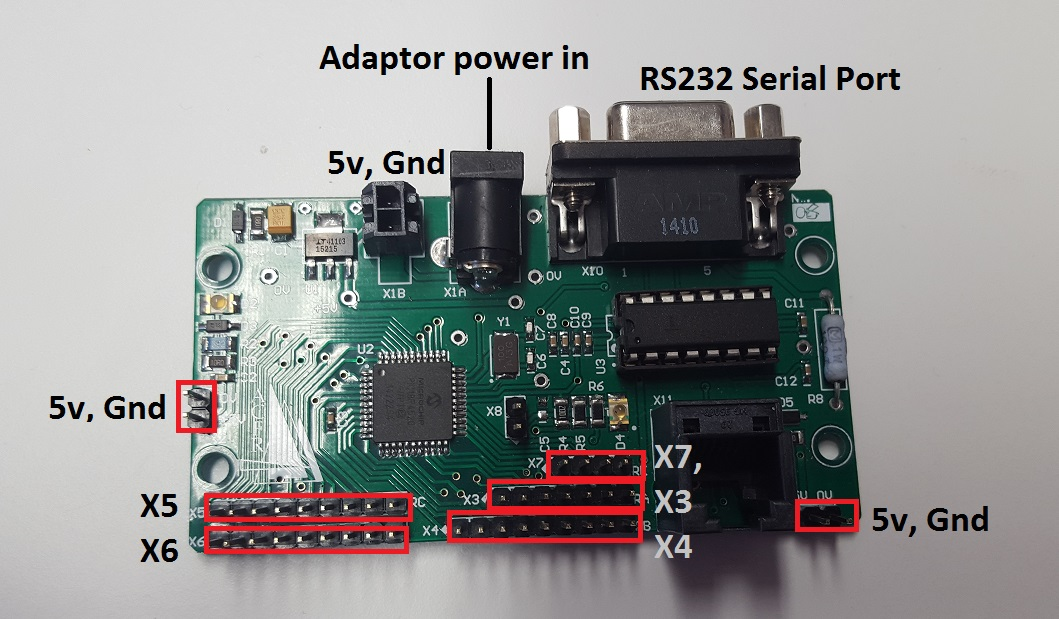
\includegraphics[width = 10cm]{pic.png}
        \caption{The MNML PIC18f4520 microcontroller}
    \end{figure}
    The PIC contains:
    \begin{itemize}
      \item 3 external interrupt sources
      \item 4 timer modules
      \item 2 CCP (capture/compare/PWM) modules
      \item
    \end{itemize}

  \subsection{Mobile Robot Hardware Design}
    \subsubsection{Power Supply}
      The Mobile Robot was powered by a Zippy Flightmax 4.2 Ahr Lithium Iron Phosphate (LiFePO4) battery. It consists of 4 series connected cells together producting a typical voltage of 12.8V. The battery is rated for a continuous discharge rate of 126A and a charge rate of 8.4A. The battery is connected to a power supply circuit that has several functions:
      \begin{enumerate}
        \item It provides a connection point for the 12.8V battery.
        \item It provides a connection point for external power supplies if the battery is removed.
        \item It provides 5V DC power at 1.5A to other hardware on the Mobile Robot.
        \item It provides a switch for turning power to the Mobile Robot off or on.
        \item It carries the Pololu 707 Dual VNH3SP30 Motor Driver board and provides power to it.
        \item It provides connection points for motor driver signals, motor leads and encoder signals.
      \end{enumerate}
      \textcolor{red}
      {
      \textit{\textbf{INSERT SCHEMATIC HERE}}
      }
    \subsubsection{Computer Design}
    Description of computer hardware, including all interface circuitry to sensors, actuators, and I/O hardware.
    \subsubsection{Sensor Hardware}
      \begin{enumerate}
        \item IR sensors:{ 3 Sharp GP2Y0A41SK0F Infrared Sensors were used to measure distance, with an effective range of 4-40cm, which corresponds to an output voltage of 0.4 to 3.1V. Exceeding 40cm, IR sensor output is saturated. There are 3 connections for the IR sensor,Vcc(nominally 5V), Gnd, and an analog output.}
        \item encoder:{ The rear motor shaft is fitted with a hall effect encoder which provides 2 square waves as outputs, one 90 degrees out of phase with the other. By measuring which signal is leading we can identify the direction of the wheel, and the frequency of the pulses tells us the speed. The sensor has 64 counts per revolution resolution.
        \begin{figure}
          \centering
          \begin{minipage}{0.45\textwidth}
              \centering
              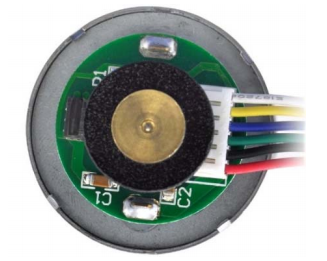
\includegraphics[width = 5cm]{encoder.png}
          \end{minipage}\hfill
          \begin{minipage}{0.45\textwidth}
              \centering
              \begin{tabular}[b]{|l|l|}
                \hline \textbf{Lead colour} & \textbf{Function}\\
                \hline Blue   & +5 V Supply\\
                \hline Green  & +0 V Supply (GND)\\
                \hline Yellow & A quadrature output signal\\
                \hline White  & B quadrature output signal\\
                \hline
              \end{tabular}
          \end{minipage}
          \caption{Encoder mounted on motor shaft, and wire functions}
        \end{figure}
        }
        \item Xbee (functions more like a sensor in robot)
      \end{enumerate}
    \subsubsection{Actuator Hardware}
      The primary actuators on the Mobile Robot were the two motors connected to the wheels. The two motors could be controlled independently allowing for turning functionality. The motor output shafts were connected to multistage planetary gearboxes having reduction ratios of 131.25:1.
      Table \ref{gearmotor} lists the acronyms and abbreviations used in this document.
      \begin{figure}[h]
        \begin{minipage}[b]{0.45\linewidth}
          \centering
          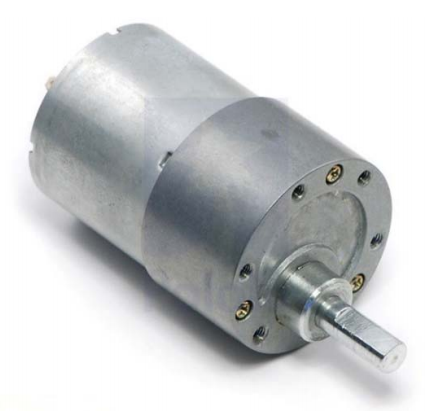
\includegraphics[width=5cm]{gearmotor.png}
        \end{minipage}\hfill
        \begin{minipage}[b]{0.45\linewidth}
          \begin{tabular}[b]{|l|l|}
            \hline \textbf{Parameter} & \textbf{Value} \\
            \hline Part number & Pololu 1447\\
            \hline No-load speed @ 12 V & 80 RPM\\
            \hline No-load current @ 12 V & 300 mA\\
            \hline Stall current @ 12 V & 5 A\\
            \hline Stall torque @ 12 V & 1.765 Nm\\
            \hline Positive terminal lead & Red\\
            \hline Negative terminal lead & Black\\
            \hline
          \end{tabular}
        \end{minipage}
        \caption{DC gearmotor and specifications}
        \label{gearmotor}
      \end{figure}
      The output shaft from the gearbox was connected to the 90mm wheel via 2 M3 screws that bore down on the shaft flat face.
    \subsubsection{Operator Input Hardware}
      The input to the Mobile Robot comes from the Commander via radio link, and as such there is no operator input hardware other than the power switch which is supplied by the power board circuit.
    \subsubsection{Operator Output Hardware}
      The operator recieves output from the Mobile Robot in the form of motion, and so the motors are an output. All other information about the state of the system is relayed via radio link to the Commander. The Mobile Robot also has a battery voltage indicator which allows for quick diagnosis of the charge level of the battery.
    \subsubsection{Hardware Quality Assurance}
      The power requirements of the Mobile Robot are regulated and met by the circuitry inside the power board. It also features a lower battery voltage cutoff of 11V to prevent the battery of excessive discharge. The IR sensor is sensitive and to stop unstable values from being read, the IR sensors were mounted onto the Mobile Robot at fixed locations. The PIC also contains brownout protection, and upon reset the code was written to keep the Mobile Robot stationary until instructed otherwise.\\

    Describe any measures that were taken to control (improve) hardware quality and reliability – Heartbeats, brownout conditioning/resets, reset conditions, testing and validation, etc.

  \subsection{Commander Hardware Design}
    \subsubsection{Power Supply}
      Unlike the Mobile Robot, the power requirements of the Commander could be fulfilled from a single 9v battery plugged into the PIC, and all power for peripheral components supplied by the PIC. Due to the many components connected to the power lines, a power rerouting circuit needed to be constructed. This circuit is shown in the next section as it involved interfacing with the PIC.
    \subsubsection{Computer Design}
    The input of the microcontroller is the joystick, from PORTA ( analog input ), there are no actuators on the commander, PORTC connect to the Xbee for the communication.\\
    \begin{document}
    
      includegraphics{commander circuit interface}
      commander circuit interface.
      \end{document}
      Description of computer hardware, including all interface circuitry to sensors, actuators, and I/O hardware.
    \subsubsection{Sensor Hardware}
    \subsubsection{Actuator Hardware}
      There was no actuating hardware present on the Commander, however, the Xbee hardware served as a means of communication between Commander and Mobile Robot.
    \subsubsection{Operator Input Hardware}
      Input hardware consisted of a 2 axis joystick, which is 2 potentiometers at mounted right angles to each other. This joystick also contains a button that can be used by depressing the joystick. A second, separate button was used on the commander for starting and stopping the mobile robot. The commander also included a master power switch.
    \subsubsection{Operator Output Hardware}
      The main output hardware consisted of an LCD screen which displayed the state of the system, as well as basic information about the Mobile Robot to to the operator. 3 LEDs were also in the original design, a power indicator, a radio link integrity indicator, and an LED to indicate the Mobile Robot was in Autonomous mode, however these LED indicators were not implemented in the final product.
    \subsubsection{Hardware Quality Assurance}
      The main hardware quality assurance policy was implemented on the PIC, with a brownout detector enabled by default on the microcontroller.\\

  \subsection{Hardware Validation}
    Details of any systematic testing to ensure that the hardware actually functions as intended.
    \subsubsection{Commander}
    Testing the commander by using LCD display first to make sure the desired outputs are correct, then send the outputs via
    xbee to verify if the outputs are still correct. \\
    Joystick should systematic testing with the mobile robot first, then connect it to the commander\\
    \subsubsection{Mobile Robot}
    Before attaching the IR sensor into the minimal board, connect it to the demo board fist and test its output analog          voltage whether it match the desire output. Once it was done, combine the IR sensor module and Xbee module, send the IR      data via xbee and verify if the IR data are correct after it transmits via xbee.\\
    In order to test the PWM motor if it actually functions as intended, attach the joystick direct to the robot minimal board, it can isolate the serial module and test the PWM motor hardware only. \\

  \subsection{Hardware Calibration Procedures}
    Procedures for calibration required in the factory, or in the field.
    \subsubsection{Commander}
    \subsubsection{Mobile Robot}

  \subsection{Hardware Maintenance and Adjustment}
    Routine adjustment and maintenance procedures.
    \subsubsection{Commander}
    \subsubsection{Mobile Robot}


\end{document}
